\ifdefined\roadmapobjectivesembedded
\else
\documentclass[10pt]{article}
\usepackage[margin=0.7in]{geometry}
\usepackage[T1]{fontenc}
\usepackage{lmodern}
\usepackage{enumitem,multicol,microtype}
\usepackage{amsmath,amssymb}
\usepackage{booktabs,tabularx,array,tikz}
\usetikzlibrary{positioning,arrows.meta}
\usepackage[hidelinks]{hyperref}
\setlength{\parindent}{0pt}
\setlength{\parskip}{3pt}
\setlength{\emergencystretch}{1.5em}
\setlist[enumerate]{leftmargin=*,itemsep=5pt,topsep=3pt,parsep=0pt}
\setlist[itemize]{leftmargin=*,itemsep=3pt,topsep=3pt,parsep=0pt}
\begin{document}
\fi

\makeatletter
\renewcommand{\section}{\@startsection{section}{1}{0pt}{8pt}{4pt}{\normalfont\large\bfseries}}
\renewcommand{\subsection}{\@startsection{subsection}{2}{0pt}{6pt}{3pt}{\normalfont\normalsize\bfseries}}
\makeatother
\setlist[itemize]{leftmargin=*,itemsep=3pt,topsep=3pt,parsep=0pt}

\begin{center}
{\large\bfseries Three Research Objectives: Paper Trails, Gaps and Methodology}\\[3pt]
{\small Placement-Aware Dynamic Graph Learning for Robust Wearable HAR}\\[3pt]
{\small Prabhat Kumar --- 2022-IMT-086 --- updated 5 October 2026}
\end{center}

\textbf{Status and revision:} Summer work is reported completed; all three objectives below are \emph{proposed}. This plan replaces the previous eight-objective list and the earlier optional-FedAvg framing. Baseline auditing, data preparation, ablations, efficiency measurement and reproducibility remain required \emph{work packages}, not additional research objectives. Federated learning is now the third objective, developed after the first two.

\section*{Exactly three research objectives}
\begin{enumerate}[label=\textbf{O\arabic*.}]
\item \textbf{Develop and evaluate placement-aware residual dynamic inter-sensor routing.} Replace the inherited fixed anatomical graph with physical, globally learned and input-dependent branches; test whether this reduces real-placement macro-F1 degradation beyond fixed graphs, augmentation and DynamicWHAR.
\item \textbf{Develop and evaluate rotation-stable representations for dynamic inter-sensor routing.} Form simple per-IMU magnitude/dot-product features before cross-sensor affinity estimation; test whether stable edges under independent mounting rotations improve the robustness--accuracy--cost trade-off over raw-axis routing and invariant fixed fusion.
\item \textbf{Develop and evaluate federated placement-robust learning across heterogeneous users.} Train the O1/O2 system using subject-specific clients without centrally pooling their raw recordings; test whether its placement robustness survives decentralized training and whether client-local normalization helps under feature-distribution shift.
\end{enumerate}

\textbf{One connected research story:} O1 asks \emph{which sensors should exchange information?} O2 asks \emph{can that exchange avoid reacting to arbitrary sensor axes?} O3 asks \emph{can the same representation be learned collaboratively when users' recordings remain local?} These are successive questions about the same wearable model, not three unrelated projects.

\subsection*{A small, targeted paper set}
Your core method-paper reading trail now uses only \textbf{DynamicWHAR, 2s-AGCN (already completed) and FedHealth~2}. O2 uses elementary magnitudes and dot products rather than an advanced equivariant encoder. Add the \textbf{REALDISP dataset documentation}; the two optional rotation references support simple features/augmentation, not extra full-paper assignments.

\begingroup
\small
\renewcommand{\arraystretch}{1.22}
\begin{tabularx}{\linewidth}{@{}>{\raggedright\arraybackslash}p{0.25\linewidth}>{\raggedright\arraybackslash}p{0.14\linewidth}X@{}}
\toprule
\textbf{Paper} & \textbf{Role} & \textbf{Why it belongs in the trail}\\
\midrule
DynamicWHAR, 2022~\cite{omdynamic} & O1 & Existing dynamic wearable interaction; the external control, not a novelty claim.\\
2s-AGCN, 2019~\cite{omagcn} & O1 design & Physical/global/sample-adaptive graph principles; skeleton inputs differ from IMUs.\\
Ba\~nos et al., 2014~\cite{ombanos} & O1/O2/O3 & Recorded ideal/self/induced placement and the distinction between rotation and physical displacement.\\
Magnitudes / dot products & O2 & Elementary rotation-invariant features; a magnitude baseline is discussed by Yurtman and Barshan~\cite{omyurtman}.\\
FedAvg, 2017~\cite{omfedavg} & O3 baseline & Local training followed by sample-size-weighted model aggregation.\\
FedHealth 2, 2021~\cite{omfedhealth} & O3 trail & Wearable personalization through client similarity and client-local batch normalization.\\
\bottomrule
\end{tabularx}
\endgroup

\textbf{Gap language used here:} ``Not established for our stated protocol'' is a testable project/evaluation gap. It is \emph{not} equivalent to ``no previous paper has done this.'' The candidate mechanism must still pass a focused prior-art check and matched experiments before any novelty or superiority claim.

\clearpage
\section*{O1. Placement-aware residual dynamic graph}
\subsection*{How this objective is chosen: the paper trail}
The inherited summer system supplies a fixed-graph starting point and sensor-drop experience, but not completed evidence for the proposed cross-placement task. DynamicWHAR already learns dynamic wearable inter-sensor correlations and provides an author implementation~\cite{omdynamic}. Therefore, the next step is \emph{not} to claim the first dynamic wearable graph, but to test a controlled change to the inherited spatial module.

The graph design follows the physical/global/sample-adaptive principle of 2s-AGCN~\cite{omagcn}. Its skeleton-action setting motivates a construction, not misplaced-IMU performance. Ba\~nos et al. supplies the reason to test that construction on recorded placement changes instead of only synthetic dead sensors~\cite{ombanos}.

\textbf{Trail in words:} inherited fixed graph $\rightarrow$ existing dynamic wearable interactions $\rightarrow$ residual topology with an anatomical prior $\rightarrow$ matched real-placement evaluation.

\subsection*{The specific gap and question}
\textbf{Candidate gap:} The value of a physical prior plus sample-dependent routing has not been established for the inherited model under the proposed held-out-subject REALDISP protocol, particularly after correcting preprocessing, augmentation and aggregation-scale confounds. This is narrower than saying that all graphs are static.

\textbf{Question:} Does residual routing improve shifted macro-F1 beyond a normalized fixed graph, fixed graph with rotation/dropout augmentation, and matched DynamicWHAR, without an unacceptable ideal-placement loss or inference penalty?

\subsection*{Proposed mechanism and controlled implementation}
For an encoded window, let $H_t\in\mathbb{R}^{N\times d}$ contain features of $N$ IMUs at encoded time $t$, with width $d$. Let $m_j\in\{0,1\}$ denote sender availability; zero unavailable features to obtain $\widehat H_t$. Form sample affinity
\[
C_t=\operatorname{softmax}_{\mathrm{row}}
\left(\frac{(\widehat H_tW_Q)(\widehat H_tW_K)^{\top}}{\tau\sqrt{d_a}}\right),
\]
where $W_Q,W_K\in\mathbb{R}^{d\times d_a}$ are learned projections, $d_a$ is their output width and $\tau>0$ a temperature. Combine branches, remove diagonal edges and mask missing senders:
\[
S_{t,ij}=m_j(1-\mathbf{1}_{i=j})
\left(\alpha A_{\mathrm{phys},ij}+\beta A_{\mathrm{global},ij}+\gamma C_{t,ij}\right),
\qquad
A_{t,ij}=\frac{S_{t,ij}}{\max\!\left(\varepsilon,\sum_{k=1}^{N}S_{t,ik}\right)}.
\]
$i$ receives and $j$ sends. $A_{\mathrm{phys}}$ is a nonnegative anatomical prior; $A_{\mathrm{global}}$ is a nonnegative learned matrix; $\alpha,\beta,\gamma\geq0$ sum to one and initially favor the physical branch. The indicator removes self-edges; $\varepsilon>0$ protects empty rows. Use a separate residual self-path in weighted message passing. Empty neighborhoods send zero messages; all sensors missing requires abstention. Availability is not a reliability estimate for a present, displaced sensor.

Keep the temporal architecture, classifier, channels, optimizer and training budget matched across variants; retrain each under the common recipe. Input affinities change at inference, but model weights are not retrained for each test window. Test finite normalization and gradients through weighted edges.

\subsection*{Deliverables and evidence required}
\begin{itemize}
\item \textbf{Runnable spatial module:} fixed, global-only, dynamic-only and residual-mixture variants with availability and gradient tests.
\item \textbf{Trustworthy controls:} audited summer baseline, no-graph control, normalized-static graph, augmentation control and a reproduced/documented DynamicWHAR comparison.
\item \textbf{Evidence package:} branch/mask/GAE ablations, gate/attention diagnostics, clean and displaced macro-F1, per-class failures and batch-one overhead, all traceable to configurations and logs.
\end{itemize}
\textbf{Decision rule:} Accept a routing benefit only if it exceeds seed variation and augmentation-only gains while satisfying a validation-defined clean-performance/cost tolerance. A reproducible negative result also completes the experiment.

\clearpage
\section*{O2. Rotation-stable features for dynamic sensor routing}
\subsection*{How this objective is chosen: the paper trail}
O1 adapts edges from observed features, but a plausible failure is that axis changes alter those features even when the activity has not changed. This motivates a representation question \emph{before} the graph, rather than assuming attention automatically learns placement invariance.

Ba\~nos et al. motivates separating rotation from position change~\cite{ombanos}. Yurtman and Barshan discuss magnitudes and geometric orientation-invariant features~\cite{omyurtman}; their SVD method is \emph{not} required. This suggests a simpler O2: start with magnitudes, add within-IMU temporal dot products, and test whether these stabilize O1's routing. Rotation augmentation supplies a learned-robustness control~\cite{omum}.

\textbf{Trail in words:} dynamic edges depend on features $\rightarrow$ mounting changes rotate axes $\rightarrow$ norms/dot products cancel that rotation $\rightarrow$ test simple invariant features before inter-IMU routing.

\subsection*{The specific gap and question}
\textbf{Candidate gap:} Do simple norm/dot-product features stabilize \emph{inter-sensor affinities} and improve residual routing beyond raw-axis dynamic graphs with augmentation and invariant fixed fusion? The contribution is this controlled integration and its evidence, not the invention of rotation invariance.

\textbf{Prior-art boundary:} Orientation-invariant wearable recognition already exists~\cite{omyurtman}. A simpler implementation is a feasibility choice, not proof of novelty. Our bounded question concerns the routing/feature combination under the declared subject-independent placement protocol.

\subsection*{Proposed mechanism and why it might help}
Let $a_i(t),\omega_i(t)\in\mathbb{R}^3$ be acceleration and angular velocity. A fixed mounting rotation $R_i$ transforms both streams in IMU $i$, with $R_i^{\top}R_i=I$. A simple feature vector is
\[
u_i(t)=\left[\|a_i(t)\|_2,\ \|\omega_i(t)\|_2,\ a_i(t)^{\top}\omega_i(t),\
a_i(t)^{\top}a_i(t-\ell),\ \omega_i(t)^{\top}\omega_i(t-\ell)\right],
\]
where $\ell>0$ is a declared lag with valid preceding samples. Norms and these within-IMU dot products are invariant because $(R_iv)^{\top}(R_iw)=v^{\top}w$. Feed the scalar sequence to an ordinary encoder $\phi$ and then O1's graph. Preserve nominal sensor identity; no quaternion or equivariant network is required. See the final page for three alternatives and their limits.

\textbf{Testable reasoning:} If these features are invariant and the physical/global branches, gates and availability mask do not depend on sensor axes, then the resulting affinity and adjacency should also be unchanged by independent fixed mounting rotations. This is a conditional property to verify numerically, not evidence of better activity recognition by itself.

Preprocessing must preserve this property: use common scaling across a modality's three axes, fitted on training data or fixed by units, rather than arbitrary axis-dependent centering/scaling. Do not add raw-axis bypasses to the classifier. All matched O1/O2 controls use the same acc/gyro channels; the inherited magnetometer configuration remains a separate audit, not a hidden input advantage.

\subsection*{Deliverables and evidence required}
\begin{itemize}
\item \textbf{Integrated features:} magnitude-only and magnitude-plus-dot-product inputs feeding an ordinary per-IMU encoder; retain a raw-axis control.
\item \textbf{Invariance tests:} independent fixed per-IMU rotations; feature, adjacency and prediction consistency checks; a diagnostic for incorrect joint-fusion assumptions.
\item \textbf{Factorial ablation:} raw-axis/invariant features crossed with fixed/dynamic fusion, plus magnitude-only and augmentation controls.
\item \textbf{Robustness--cost report:} synthetic-rotation and recorded-displacement results separately, clean macro-F1, parameter count and batch-one latency/memory.
\end{itemize}
\textbf{Limits:} Rotation invariance does not remove translation effects, identify unknown body locations or guarantee robustness to time-varying mount motion. The features may discard useful directions. Use classification-only training for the principal comparison; a GAE uses invariant targets or a separate raw-axis decoder path, not exact raw reconstruction from an invariant code alone.

\clearpage
\section*{O3. Federated placement-robust learning across users}
\subsection*{How this objective is chosen: the paper trail}
The first two objectives assume a common training process. The third changes \emph{where learning occurs}: simulate one client per user, retaining that user's recordings locally. FedAvg supplies the local-update/server-aggregation baseline~\cite{omfedavg}. This is a deployment-oriented research setting, not proof that FL automatically improves accuracy or guarantees privacy.

FedHealth~2 is the key wearable trail: it uses client similarity and client-local batch normalization for personalized learning. Its reported PAMAP experiment creates 20 clients with Dirichlet-distributed labels, and the authors describe the experimental shifts as mainly label-related~\cite{omfedhealth}. That motivates testing \emph{recorded placement-induced feature shift}, rather than treating synthetic label imbalance as sufficient evidence.

The proposed extension is a test of O1/O2 under this client setting, not a claim that federated wearable recognition or graph-based FL has never existed. FedHealth~2 supplies the personalization trail; the remaining question is whether our spatial/rotation choices retain their benefit under recorded placement changes and subject-based clients.

\textbf{Trail in words:} O1/O2 placement-robust representations $\rightarrow$ FedHealth~2's wearable personalization/local normalization $\rightarrow$ test real-placement feature shift in subject-based multi-IMU clients.

\subsection*{The specific gap and question}
\textbf{Candidate gap:} The reviewed experiments do not establish whether the proposed rotation-stable anatomical routing retains its benefit under \emph{subject-client federation with recorded placement changes}, beyond a fixed/scalar graph, plain FedAvg and a client-local-normalization control.

\textbf{Question:} Does O2 reduce the federated robustness loss caused by client-specific placement conditions, and can a small personalization mechanism improve known-client performance without an unacceptable communication/compute cost? This is an inferred, bounded extension from the selected papers, not an exhaustive claim about all federated HAR research.

\subsection*{Proposed federated mechanism}
Use one training subject per client within a dataset; keep activity labels, sensor ordering and architecture aligned. For communication round $r$, each selected client starts from the shared model, trains locally for a fixed number of epochs, and returns parameters/updates. Plain FedAvg gives
\[
\theta^{(r+1)}=\sum_{k\in\mathcal S_r}
\frac{n_k}{\sum_{u\in\mathcal S_r}n_u}\,\theta_k^{(r+1)}.
\]
$\theta^{(r+1)}$ is the new server parameter vector; $\mathcal S_r$ the participating client set; $n_k$ the number of local training windows; and $\theta_k^{(r+1)}$ client $k$'s locally updated parameters. Broadcast the new shared parameters for the next round. This is a borrowed baseline, not a new aggregation equation~\cite{omfedavg}.

Compare plain FedAvg with \emph{one FedHealth-2-inspired client-local-normalization variant}; place batch normalization after invariant scalar projection, not on raw vector axes. Use identical normalization layers in both models; change only shared versus client-local state. Share graph/encoder/temporal/classifier parameters but retain local normalization state. Label this as an adaptation, not a faithful FedHealth~2 reproduction unless similarity weighting and other details are also reproduced.

\subsection*{Deliverables and two distinct evaluation tracks}
\begin{itemize}
\item \textbf{Federated simulator:} subject-client manifests, reproducible client selection, rounds/local epochs, shared-versus-local parameter definitions and no central raw-recording pooling during federated training.
\item \textbf{Unseen-user track:} held-out test and validation subjects never participate in training. Evaluate the shared model with normalization fixed from training sources; do not learn target statistics or claim personalized zero-shot inference.
\item \textbf{Known-client track:} train on each client's ideal recordings and test disjoint recordings/available placements using frozen client-local state. Keep this personalization result separate from unseen-subject generalization.
\item \textbf{Matched evidence:} local-only, centralized, FedAvg and local-normalization controls; scalar/fixed versus O1/O2 models; client macro-F1, worst-client performance, convergence, communication bytes and local training cost.
\end{itemize}
\textbf{Scope:} Simulator results do not demonstrate on-watch training or privacy. No differential-privacy guarantee is claimed. The contribution is measured placement-robustness retention under federation; report trade-offs and negative results.

\clearpage
\section*{Proposed methodology connecting all three objectives}
\subsection*{Common model and data flow}
\begin{center}
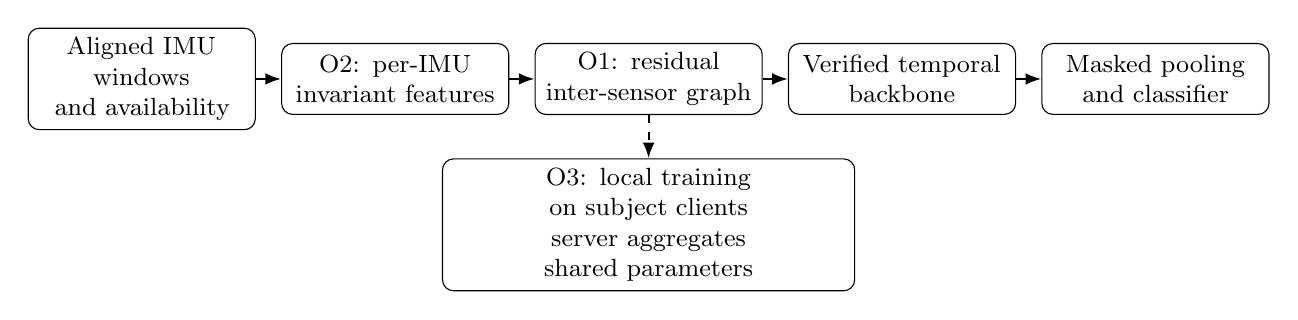
\begin{tikzpicture}[
  node distance=0.32cm,
  block/.style={draw,rounded corners,align=center,text width=2.65cm,minimum height=0.90cm,font=\small},
  arrow/.style={-{Latex[length=2mm]},thick}
]
\node[block] (input) {Aligned IMU windows\\and availability};
\node[block,right=of input] (features) {O2: per-IMU\\invariant features};
\node[block,right=of features] (graph) {O1: residual\\inter-sensor graph};
\node[block,right=of graph] (temporal) {Verified temporal\\backbone};
\node[block,right=of temporal] (head) {Masked pooling\\and classifier};
\node[block,below=0.55cm of graph,text width=5.0cm] (federation) {O3: local training on subject clients\\server aggregates shared parameters};
\draw[arrow] (input)--(features);
\draw[arrow] (features)--(graph);
\draw[arrow] (graph)--(temporal);
\draw[arrow] (temporal)--(head);
\draw[arrow,dashed] (graph)--(federation);
\end{tikzpicture}
\end{center}
Federation describes \emph{training organization}, not another inference layer. Validate O1 with scalar features, then introduce O2. In O3, compare both versions rather than assuming central gains transfer to FL.

\subsection*{Data audit and non-leaking preprocessing}
Use REALDISP for recorded placement shifts and DSADS for secondary rotation/dropout tests; do not combine incompatible sensor schemas into a single federation. Audit subject/session/scenario, sensor order, labels, units and NaNs before windowing. Start with 50-sample REALDISP windows, stride 25; validate these choices. Match channels/windows across controls; document any inherited nine-channel versus common six-channel change.

Partition subjects for unseen-user testing \emph{before} computing statistics or windows. For known-client testing, split recordings or non-overlapping time blocks with a window-length exclusion gap; keep test placements out of training/calibration. Compute any statistics only from authorized training data. Use rotation-compatible preprocessing throughout the matched O2 comparison; place synthetic rotations in raw vector space and record their severity. Distinguish whole-sensor dropout from losing only one modality.

\subsection*{Weighted graph layer and classification objective}
A graph layer can use
\[
Z_{t,i}=m_i\left[\sigma\!\left(\sum_j A_{t,ij}\widehat H_{t,j}W_g+b_g\right)
+\widehat H_{t,i}W_r\right].
\]
$Z_{t,i}$ is sensor $i$'s graph output; $W_g$ and $b_g$ transform neighbor messages; $W_r$ is the residual projection; $\sigma$ an activation; and $m_i$ the availability indicator. $A_t$ and $\widehat H_t$ are defined under O1. Remove self-neighbor edges before this layer, mask missing outputs and pool only available sensors after temporal modeling.

Use activity cross-entropy for the principal matched study. The inherited GAE remains a controlled O1 ablation, not a fourth objective: where suitable targets exist, $\mathcal L=\mathcal L_{\mathrm{cls}}+\lambda_{\mathrm{rec}}\mathcal L_{\mathrm{rec}}$, with $\lambda_{\mathrm{rec}}\geq0$. Here $\mathcal L_{\mathrm{cls}}$ is classification loss and $\mathcal L_{\mathrm{rec}}$ reconstruction error on intentionally masked known training targets. Set the weight to zero without such targets; never assume ideal/displaced recordings are aligned pairs. Revisit targets after O2's invariant bottleneck.

\subsection*{Experiments that identify each objective's contribution}
\begingroup
\small
\renewcommand{\arraystretch}{1.18}
\begin{tabularx}{\linewidth}{@{}>{\raggedright\arraybackslash}p{0.11\linewidth}>{\raggedright\arraybackslash}p{0.40\linewidth}X@{}}
\toprule
\textbf{Test} & \textbf{Matched comparison} & \textbf{Evidence sought}\\
\midrule
O1 & Fixed/normalized-static/augmentation/DynamicWHAR versus residual routing & Added value of adaptive spatial connectivity.\\
O2 & Raw-axis/norm/norm-plus-dot-product features $\times$ fixed/dynamic fusion; augmentation & Stable affinities and recognition beyond either component alone.\\
O3 & Same O1/O2 architectures under centralized/local-only/FedAvg/local-normalization training & Retained placement robustness, personalization and communication trade-offs.\\
\bottomrule
\end{tabularx}
\endgroup

\textbf{Reporting:} Measure subject/client macro-F1, paired ideal-to-shift degradation, per-class failures and seed/subject uncertainty. REALDISP induced displacement is documented for subjects 2, 5 and 15; audit files rather than inventing all-subject displaced folds~\cite{ombanos}. Report rotations, real displacement and dropout separately before combined stress. Add batch-one median/p95 inference latency, memory, parameters and window delay; O3 additionally reports rounds, bytes and local training time. Lock all tolerances/hyperparameters using validation only and retain negative results.

\clearpage
\section*{Focused references and final deliverable map}
\begingroup
\renewcommand{\refname}{Three core papers and optional/background references}
\begin{thebibliography}{99}
\ifdefined\roadmapobjectivesembedded
\setcounter{enumiv}{7}
\fi
\setlength{\itemsep}{6pt}
\setlength{\parskip}{0pt}
\raggedright

\bibitem{omdynamic} S. Miao, L. Chen, R. Hu and Y. Luo.
\href{https://doi.org/10.1145/3550331}{\emph{Towards a Dynamic Inter-Sensor Correlations Learning Framework for Multi-Sensor-Based Wearable Human Activity Recognition}}.
ACM IMWUT, vol. 6, no. 3, art. 130, 2022.
\href{https://github.com/wdkhuans/DynamicWHAR}{Official author implementation}. \textbf{Use:} O1 wearable dynamic-interaction control; the code repository uses a shortened title.

\bibitem{omagcn} L. Shi, Y. Zhang, J. Cheng and H. Lu.
\href{https://arxiv.org/abs/1805.07694}{\emph{Two-Stream Adaptive Graph Convolutional Networks for Skeleton-Based Action Recognition}}.
CVPR, 2019. \textbf{Use:} O1 topology-design foundation, with the skeleton/IMU boundary stated.

\bibitem{ombanos} O. Ba\~nos, M. A. Toth, M. Damas, H. Pomares and I. Rojas.
\href{https://doi.org/10.3390/s140609995}{\emph{Dealing with the Effects of Sensor Displacement in Wearable Activity Recognition}}.
Sensors, vol. 14, no. 6, pp. 9995--10023, 2014.
\href{https://pmc.ncbi.nlm.nih.gov/articles/PMC4118358/}{Open full text}. \textbf{Background only:} recorded-placement problem/protocol; no additional full-paper reading is assigned for today.

\bibitem{omyurtman} A. Yurtman and B. Barshan.
\href{https://doi.org/10.3390/s17102222}{\emph{Activity Recognition Invariant to Sensor Orientation with Wearable Motion Sensors}}.
Sensors, vol. 17, no. 10, art. 2222, 2017.
\textbf{Optional:} Section 2's magnitudes and Section 3.1's geometric features; the SVD method is not required reading.

\bibitem{omum} T. T. Um et al.
\href{https://arxiv.org/abs/1706.00527}{\emph{Data Augmentation of Wearable Sensor Data for Parkinson's Disease Monitoring using Convolutional Neural Networks}}.
ICMI, 2017, \href{https://doi.org/10.1145/3136755.3136817}{doi:10.1145/3136755.3136817}.
\textbf{Optional:} rotation-augmentation background, not proof of our independent-IMU or real-placement robustness.

\bibitem{omfedavg} H. B. McMahan, E. Moore, D. Ramage, S. Hampson and B. A. y Arcas.
\href{https://proceedings.mlr.press/v54/mcmahan17a.html}{\emph{Communication-Efficient Learning of Deep Networks from Decentralized Data}}.
AISTATS, PMLR 54, pp. 1273--1282, 2017.
\textbf{Background only:} O3's aggregation equation and communication accounting; no additional full-paper reading is assigned for today.

\bibitem{omfedhealth} Y. Chen, W. Lu, J. Wang and X. Qin.
\href{https://arxiv.org/abs/2106.01009}{\emph{FedHealth 2: Weighted Federated Transfer Learning via Batch Normalization for Personalized Healthcare}}.
arXiv:2106.01009, 2021.
\href{https://federated-learning.org/fl-ijcai-2021/FTL-IJCAI21_paper_4.pdf}{Author workshop paper}.
\textbf{Use:} wearable personalization/local-normalization trail; inspect Section 4's client construction and ablations.

\bibitem{omrealdisp} O. Ba\~nos, M. Toth and O. Amft.
\href{https://archive.ics.uci.edu/dataset/305/realdisp+activity+recognition+dataset}{\emph{REALDISP Activity Recognition Dataset}}.
UCI Machine Learning Repository, dataset 305, \href{https://doi.org/10.24432/C5GP6D}{doi:10.24432/C5GP6D}.
The repository's citation uses 2012; its donation date is 24 July 2014. \textbf{Use:} dataset metadata, file listing and raw format, not another method-paper assignment.

\end{thebibliography}
\endgroup

\subsection*{What is delivered for each of the three objectives?}
\begingroup
\small
\renewcommand{\arraystretch}{1.22}
\begin{tabularx}{\linewidth}{@{}>{\raggedright\arraybackslash}p{0.11\linewidth}>{\raggedright\arraybackslash}p{0.40\linewidth}X@{}}
\toprule
\textbf{Goal} & \textbf{Technical artifact} & \textbf{Research evidence}\\
\midrule
O1 & Weighted residual graph, tested masks, audited baseline and spatial variants. & Matched real-placement results, branch/GAE ablations and inference overhead.\\
O2 & Norm/dot-product features and ordinary encoder integrated with routing; invariance checks. & Raw-axis/invariant $\times$ fixed/dynamic comparison, rotation consistency and displacement/cost trade-offs.\\
O3 & Subject-client FL simulator, FedAvg and a clearly specified local-normalization adaptation. & Separate unseen-user/known-client results, client variability, convergence, communication and training cost.\\
\bottomrule
\end{tabularx}
\endgroup

\textbf{Feasible sequence:} Establish O1 and the leakage-free protocol first; develop O2 as the single representation extension; then evaluate O3 using the same frozen model choices. Use REALDISP first and DSADS second. Simulator access, compatible implementations and validation evidence are prerequisites, not assumed completed milestones.

\textbf{Defensible final gap statement:} ``We propose to test residual inter-sensor routing built from rotation-stable per-IMU features, and determine whether its benefits under recorded placement shifts persist in subject-based federated training beyond matched fixed-graph, augmentation, invariant-fusion and federated controls.'' This is the research question supported by the trail; any claim of firstness or guaranteed gain requires further evidence.

\clearpage
\section*{Clarification: does O2 collide with the earlier generative autoencoder?}
\textbf{Short answer:} Not automatically. Reconstruction and rotation stability ask different questions, even if both reuse an encoder. However, \emph{exact raw-axis reconstruction from a strictly invariant code can conflict with O2}. Compatibility depends on the decoder's target and inputs, not the label ``generative.''

\subsection*{What changes, and what remains from the summer work?}
Your \href{colloquium_report.pdf}{Summer Colloquium report}, as summarized in the prepared report, describes GAE reconstruction with sensor-drop training. Keep it as the starting point. Check whether the decoder targets raw sensor values, adjacency or other features: compatibility depends on that target. ``Generative'' does not establish rotation invariance or a particular probabilistic architecture.

\begingroup
\small
\renewcommand{\arraystretch}{1.15}
\begin{tabularx}{\linewidth}{@{}>{\raggedright\arraybackslash}p{0.17\linewidth}>{\raggedright\arraybackslash}X>{\raggedright\arraybackslash}X@{}}
\toprule
\textbf{Aspect} & \textbf{Earlier GAE work} & \textbf{Proposed O2}\\
\midrule
Question & Can reconstruction/sensor-drop training improve recognition with missing inputs? & Can independent mounting rotations leave recognition features and inter-sensor affinities stable?\\
Input condition & A sensor or training target is masked. & A sensor remains active but its vector axes are rotated.\\
Learning target & Recover the implemented graph/sensor target. & Preserve activity information while removing local orientation dependence before routing.\\
Evidence & Reconstruction and missing-sensor recognition ablations. & Rotated-input feature/edge consistency and matched rotation/displacement recognition tests.\\
\bottomrule
\end{tabularx}
\endgroup

\subsection*{When would O2 overlap with the previous contribution?}
A reconstruction loss may improve robustness, but does not establish rotation invariance. O2 now uses directly checkable norm/dot-product features. If your earlier model already enforced independent per-IMU invariance and tested stable edges under the same rotation protocol, narrow O2's claim; adding another autoencoder is not a distinct contribution.

\subsection*{The real architectural conflict: which information must the latent code retain?}
For one IMU window $X$ and a rotation $R$, strict invariance requires
\[
f(R\cdot X)=f(X)=z.
\]
Here $f$ is the classification-feature encoder, $R\cdot X$ the rotated window and $z$ its invariant code. A deterministic decoder $D$ receiving only $z$ has one output $D(z)$. If $R\cdot X\neq X$, that output cannot equal \emph{both} raw-axis windows exactly. This is an information-loss argument, not a claim that autoencoders cannot learn useful invariant features. A generative decoder can sample orientations but cannot identify the observed one from the same invariant code alone. The conflict does \emph{not} automatically apply to orientation-independent graph or scalar targets.

\subsection*{How to retain the earlier work without creating this conflict}
\begin{itemize}
\item \textbf{Clean principal comparison:} keep the old GAE model as a baseline; train matched raw-axis/invariant O2 variants with classification only. Temporarily disabling its auxiliary decoder does not erase the completed summer contribution.
\item \textbf{Compatible reconstruction ablation:} reconstruct invariant targets, such as vector norms or dot products \emph{within the same IMU}. Check graph targets separately; raw dot products across independently rotated IMUs are not generally invariant.
\item \textbf{If raw axes must be reconstructed:} retain a separate orientation-sensitive path from the raw inputs, or valid orientation conditioning. Do not send that path to the invariant classifier/routing module or attach the unchanged raw decoder to invariant features and assume compatibility.
\end{itemize}

\textbf{Evidence that O2 adds something:} compare the inherited GAE, rotation-augmented GAE and matched O2 variants under identical inputs/splits/backbone/budgets. Report rotation macro-F1, feature/adjacency consistency, dropout results separately and inference cost. Adding invariant-target reconstruction is an ablation within O2, not a fourth objective.

\textbf{Presentation-ready explanation:} ``My earlier GAE studied reconstruction and missing sensors. O2 studies active sensors with changed axes and tests orientation-stable routing. I retain the GAE as a baseline, adapting its decoder where needed. O2's added value requires matched evidence.''

\clearpage
\section*{One-day reading plan: three core papers and simple O2 mathematics}
\textbf{Today's goal:} Explain the chain \emph{what exists $\rightarrow$ what is not established for our task $\rightarrow$ problem statement $\rightarrow$ O1/O2/O3}. Do not reproduce models overnight or read every equation. The numbered points below are preparation steps, not additional objectives.

\begin{enumerate}[label=\textbf{\arabic*.},itemsep=5pt]
\item \textbf{Use this order and time budget.} Refresh \textbf{2s-AGCN for 15 minutes}; read \textbf{DynamicWHAR for 90 minutes} and \textbf{FedHealth~2 for 90 minutes}. Spend \textbf{45 minutes on the final-page O2 alternatives}, not an advanced encoder paper. Prioritize introductions, architecture and evaluation; leave implementation details for later.

\item \textbf{Take the same five notes for each paper.} Write: \emph{problem; mechanism; inputs/fusion; actual evaluation; our remaining question}. Attach a page/section to each factual note. Mark your own gap inference separately. A difference between architectures is a reason to investigate, not evidence that your model is better.

\item \textbf{DynamicWHAR $\rightarrow$ why O1?} Understand per-sensor features and learned inter-sensor interaction~\cite{omdynamic}. Check the exact subject/placement protocol; a dataset name alone does not establish placement robustness. \emph{Our next question:} does residual anatomical routing help our inherited system under matched real-placement shifts beyond existing dynamic interaction? \textbf{Output:} one architecture sketch and one bounded O1 gap sentence; never claim that wearable dynamic graphs do not exist.

\item \textbf{2s-AGCN $\rightarrow$ how O1 is designed.} Review only its physical, global and sample-adaptive graph components~\cite{omagcn}. Explain why preserving an anatomical prior while learning corrections is a reasonable hypothesis. Its skeleton inputs do not prove misplaced-IMU performance. \textbf{Output:} a one-minute explanation of the three graph branches and their ablations. The formula is borrowed design inspiration, not your novelty claim.

\item \textbf{Simple rotation mathematics $\rightarrow$ why O2?} Work through $R^{\top}R=I$, preservation of norms and preservation of within-IMU dot products on the final page. These are established mathematical facts, not a novelty claim. \emph{Our question:} do these features stabilize O1's affinities beyond augmentation and invariant fixed fusion? \textbf{Output:} the raw-axis/invariant $\times$ fixed/dynamic comparison; optional references do not add full-paper reading.

\item \textbf{FedHealth~2 $\rightarrow$ why O3?} Read the method and experimental setup, especially client similarity, local batch normalization and PAMAP client construction~\cite{omfedhealth}. Distinguish label imbalance from placement-induced feature shift. \emph{Our next question:} does the O1/O2 model retain placement robustness in subject-client federation beyond shared training and local-normalization controls? \textbf{Output:} one client/server sketch and separate unseen-user versus known-client tests. Do not claim FL itself is new or guarantees privacy.

\item \textbf{Turn the notes into one problem statement and three objectives.} After reading, say: ``Existing papers motivate adaptive interactions, rotation-stable features and wearable personalization. Their joint benefit for our inherited system under a matched real-placement/subject-client protocol is not established.'' \textbf{Problem:} robust multi-IMU activity recognition despite orientation/placement changes and user heterogeneity, including decentralized training. \textbf{Objectives:} O1 tests routing; O2 tests orientation-stable features for that routing; O3 tests retention of those benefits under federation. This is a candidate gap inferred from the selected papers, not proof of global firstness.

\item \textbf{Finish with communication, not coding.} Core papers take \textbf{3 hours 15 minutes}; add \textbf{45 minutes each for O2 mathematics and REALDISP}: \textbf{4 hours 45 minutes}. Add \textbf{1 hour} for the evidence/gap matrix, \textbf{1 hour} for slides and \textbf{45 minutes} for rehearsal: \textbf{7 hours 30 minutes plus breaks}. Prepare literature, gap-to-objective and pipeline slides; label all new experiments proposed.
\end{enumerate}

\clearpage
\section*{Clickable paper links and REALDISP reading sources}
\textbf{How to use this page:} Open one full-text version per selected paper. The links are clickable in the PDF; visible URLs can also be copied. Keep your existing paper order and use the dataset-specific sources below rather than adding more method papers.

\begin{enumerate}[label=\textbf{\arabic*.},itemsep=7pt]
\item \textbf{DynamicWHAR --- the O1 wearable interaction reference.}\\
\emph{Towards a Dynamic Inter-Sensor Correlations Learning Framework for Multi-Sensor-Based Wearable Human Activity Recognition}~\cite{omdynamic}.\\
Publisher/DOI: \url{https://doi.org/10.1145/3550331}\\
Official author code and architecture figures: \url{https://github.com/wdkhuans/DynamicWHAR}\par
Read feature extraction, information interaction and evaluation. The repository includes REALDISP configurations, so the gap is \emph{not} simply using REALDISP. Inspect placement conditions and splits. ACM full text may require institutional access; the repository supports reading but is not a replacement for the paper.

\item \textbf{2s-AGCN --- already read; refresh its graph construction only.}\\
\emph{Two-Stream Adaptive Graph Convolutional Networks for Skeleton-Based Action Recognition}~\cite{omagcn}.\\
Paper page: \url{https://arxiv.org/abs/1805.07694}\\
PDF: \url{https://arxiv.org/pdf/1805.07694}\par
Spend 15 minutes revisiting the physical/global/sample-dependent branches and the skeleton-input boundary. Do not reread the entire paper or claim the borrowed adjacency principle as a new invention.

\item \textbf{O2 --- simple mathematics, with optional background only.}\\
Geometric features: \href{https://doi.org/10.3390/s17102222}{Yurtman and Barshan, Sections 2 and 3.1 only}~\cite{omyurtman}.\\
Rotation augmentation: \href{https://arxiv.org/abs/1706.00527}{Um et al., author paper}~\cite{omum}.\par
Neither is a new full-paper assignment. Skip the SVD method; use the final-page proofs and proposed norm/dot-product features. Augmentation is an empirical control, not exact invariance.

\item \textbf{FedHealth 2 --- the O3 personalization reference.}\\
\emph{FedHealth 2: Weighted Federated Transfer Learning via Batch Normalization for Personalized Healthcare}~\cite{omfedhealth}.\\
Paper page: \url{https://arxiv.org/abs/2106.01009}\\
PDF: \url{https://arxiv.org/pdf/2106.01009}\par
Alternative: \href{https://federated-learning.org/fl-ijcai-2021/FTL-IJCAI21_paper_4.pdf}{click for the 7-page author workshop PDF}. Choose one version and record it in your notes. Prioritize client similarity, local batch normalization and the activity-recognition experiment, rather than the separate diagnosis application.

\item \textbf{REALDISP --- official dataset page and placement documentation.}\\
Repository description, file listing and download button:\\
\url{https://archive.ics.uci.edu/dataset/305/realdisp+activity+recognition+dataset}\par
Dataset DOI: \url{https://doi.org/10.24432/C5GP6D}\par
Placement explanation: \href{https://pmc.ncbi.nlm.nih.gov/articles/PMC4118358/}{Ba\~nos et al.: open full text, especially Sections 3--4 and Figures 2--5}~\cite{ombanos,omrealdisp}. This is targeted dataset reading, not an additional full method-paper assignment. Read the UCI description first, then the scenario/coverage explanation.

\item \textbf{Spend 45 minutes on the dataset, not the entire download.} Use 15 minutes for UCI metadata/format, 20 minutes for placement scenarios and coverage, and 10 minutes to draft the feature/split checklist. The UCI page lists a 2.5\,GB archive; do not make completing that download a prerequisite for today's proposal preparation. Mark file-level checks as pending until inspected.
\end{enumerate}

\clearpage
\section*{REALDISP: important points to understand and present}
\textbf{Sources:} the official UCI dataset description~\cite{omrealdisp} and the recorded-placement study~\cite{ombanos}. The protocol choices below are \emph{our proposed evaluation}, not claimed reproductions of every published split.

\begin{enumerate}[label=\textbf{\arabic*.},itemsep=4pt]
\item \textbf{Know the basic setup.} REALDISP means realistic sensor displacement. It includes \textbf{17 subjects, 9 IMUs, 33 activities and 50\,Hz sampling}; UCI lists \textbf{47 files}. Activities include warm-up/fitness exercises, not only walking and sitting. These are dataset-level counts, not a guarantee that every subject has every activity/scenario.

\item \textbf{Know the sensor identities before drawing the graph.} The nominal order is \textbf{S1 left calf; S2 left thigh; S3 right calf; S4 right thigh; S5 back; S6 left lower arm; S7 left upper arm; S8 right lower arm; S9 right upper arm}. Preserve that order in feature extraction and the anatomical prior; do not assume node identities can be inferred automatically after relocation.

\item \textbf{Understand one raw row.} There are \textbf{120 columns}: two timestamp fields, nine 13-channel IMU blocks and one activity label. Each block contains three acceleration, three gyroscope and three magnetic-field components plus four quaternion components: $2+9(3+3+3+4)+1=120$. Timestamps/labels are not activity input features. Verify units and conventions before parsing or using quaternions.

\item \textbf{Separate the three placement scenarios.} \emph{Ideal:} an instructor attaches sensors at the intended locations. \emph{Self:} users attach a subset themselves. \emph{Induced:} an instructor intentionally introduces rotations/translations. Files can use the word \texttt{mutual}, such as \texttt{subject15\_mutual5.log}; map file names to documented induced conditions, not a fourth invented scenario.

\item \textbf{Audit coverage, not just the subject total.} Induced displacement is documented for \textbf{subjects 2, 5 and 15}. The study also reports missing activity coverage, including self-placement data for subjects 6 and 13 and very little ideal activity data for subject 7. Confirm the downloaded release; do not plan 17 valid induced folds or confuse file presence with usable labelled activities.

\item \textbf{Do not confuse displacement with missing sensors or paired reconstruction.} Displaced sensors remain active; a binary availability mask cannot identify their reliability. Ideal/self/induced runs are separate recordings, not automatically time-aligned clean/corrupted targets. Rotation invariance does not guarantee robustness to translations or arbitrary body-location changes.

\item \textbf{Validate columns and labels before modeling.} The UCI prose column list contains an extra \texttt{Gyr} entry and an inconsistent S7 range; verify the 13-channel blocks against package documentation/sample rows. Check background/transition label handling, timestamps and invalid values. A catalog ``instance'' count is not our declared window count; calculate rows and valid windows during the file audit.

\item \textbf{Declare our matched input and windows.} The principal O1/O2 comparison uses acc/gyro only: $[T,N,F]=[50,9,6]$, where $T$ is samples, $N$ sensors and $F$ features per sensor. At 50\,Hz, this is a one-second window with stride 25, or a half-second step. These are proposed starting settings, not official mandatory windows; keep all controls matched. Report the inherited nine-feature input separately.

\item \textbf{Explain the subject-independent split clearly.} Train on other subjects' ideal recordings, hold out separate validation/test subjects, and test available placements of the unseen subject. Split before overlapping windows and fit preprocessing on training data only. Rotate raw vectors before rotation-compatible scaling. Declare window-label rules and class exclusions; never tune on test placement scores.

\item \textbf{Connect the dataset to the three objectives.} \textbf{O1:} test whether adaptive inter-sensor routing helps under recorded shifts. \textbf{O2:} test independent rotations separately from recorded displacement. \textbf{O3:} simulate training subjects as clients and test retained robustness under federation; REALDISP was not itself collected as an FL experiment. Keep known-client personalization separate from unseen-subject testing.

\item \textbf{Prepare evidence, not invented counts.} Draft a manifest with subject, recording/scenario, nominal sensor order, valid labels, usable rows and exclusions. Compare methods on the same available subject--scenario/class sets; report macro-F1 and ideal-to-shift degradation with uncertainty. With only three induced subjects, conclusions are limited. Today's deliverable is one dataset slide and a documented protocol/checklist; raw-file statistics remain pending until audited.
\end{enumerate}

\clearpage
\begingroup
\setlist[itemize]{leftmargin=*,itemsep=2pt,topsep=2pt,parsep=0pt}
\section*{What to highlight in each paper: an objective-focused reading map}
\textbf{Mark these parts in your PDFs.} Highlight \emph{the problem, mechanism and evaluation}; write our remaining question separately. Bold locators identify priority reading, not new objectives. Numbers follow the linked arXiv texts, except FedHealth~2's seven-page workshop version.

\subsection*{1. DynamicWHAR: establish what already exists before proposing O1}
\begin{itemize}
\item \textbf{Highlight: Introduction, architecture overview, Initial Feature Extraction and Dynamic Information Interaction.} Trace how each sensor becomes a feature and how information moves between sensors~\cite{omdynamic}. These module names are confirmed in the author repository; locate their descriptions in the publisher PDF rather than guessing section/page numbers.
\item \textbf{Read carefully: experimental setup, interaction ablations and any availability tests.} Record sensors, subject splits, placement conditions and controls actually tested. The code includes REALDISP; merely selecting that dataset is not a gap.
\item \textbf{Explain for O1:} ``Dynamic wearable interaction already exists. I will test whether an anatomical-prior residual mixture improves our inherited model under matched real-placement shifts.'' Sketch the existing interaction versus our physical/global/input-dependent branches. Skim routine training settings today, but retain the evaluation protocol.
\end{itemize}

\subsection*{2. 2s-AGCN: refresh only the graph-design evidence for O1}
\begin{itemize}
\item \textbf{Highlight: Section 4.1, Adaptive Graph Convolutional Layer, and Figure 2.} Annotate $A_k$, $B_k$ and $C_k$: physical connectivity, globally learned connectivity and sample-specific connectivity. Review the embedding/softmax construction of $C_k$~\cite{omagcn}.
\item \textbf{Check: Section 5.3, Ablation Study.} Identify which graph components are compared; do not infer wearable-placement gains from skeleton-action results. Section 4.3's joint/bone streams are secondary for our IMU proposal.
\item \textbf{Explain for O1:} ``This supplies the design trail, not my novelty. I adapt its graph principle to IMUs and test branch contributions and placement robustness.'' Since you have completed it, use only the planned 15-minute refresh.
\end{itemize}

\subsection*{3. O2 mathematics: no advanced encoder paper required}
\begin{itemize}
\item \textbf{Highlight: the final-page norm and dot-product proofs.} Use Yurtman and Barshan's Sections 2 and 3.1 only if needed~\cite{omyurtman}; skip SVD. Within-IMU temporal dot products add information that magnitudes discard.
\item \textbf{Read carefully: exact versus approximate invariance.} Norm/dot-product features cancel fixed rotations algebraically; rotation augmentation encourages robustness through training~\cite{omum}. Neither establishes arbitrary translation robustness.
\item \textbf{Explain for O2:} ``I test lightweight invariant features before routing, beyond augmentation and invariant fixed fusion.'' Keep sensor identity, use raw-axis controls, and measure both recognition and feature/edge consistency. No claim of firstness follows from simplifying the encoder.
\end{itemize}

\subsection*{4. FedHealth 2: connect wearable personalization to O3}
\begin{itemize}
\item \textbf{Highlight: Sections 3.1--3.4 and Figure 2.} Focus on feature alignment, local batch normalization, client-similarity weighting and the federated training flow. Separate the complete paper method from our simpler local-normalization control~\cite{omfedhealth}.
\item \textbf{Read carefully: Section 4.1, Activity Recognition, and Figure 4.} Mark PAMAP client construction, train/test division and weighting/normalization comparisons. The workshop version creates 20 clients with Dirichlet label partitions, not 20 independent subjects. Skim Section 4.2's Parkinson diagnosis experiment; do not mix version-specific protocols.
\item \textbf{Explain for O3:} ``Wearable federation and personalization already exist. I will test whether O1/O2 placement robustness survives subject-client federation, distinguishing known-client personalization from unseen-user generalization.'' Label imbalance alone does not test placement-induced feature shift; local data does not establish a formal privacy guarantee.
\end{itemize}

\textbf{REALDISP companion:} Highlight UCI's format/scenarios and Ba\~nos et al., Sections 3--4/Figures 2--5~\cite{omrealdisp,ombanos}; use the preceding coverage checklist. \textbf{Final slide:} evidence $\rightarrow$ remaining question $\rightarrow$ O1/O2/O3. These are candidate gaps, not proof of novelty.
\endgroup

\clearpage
\begingroup
\setlist[enumerate]{leftmargin=*,itemsep=5pt,topsep=3pt,parsep=0pt}
\section*{Proposed O2 alternatives: simple mathematics for sensor rotation}
\textbf{Revised plan:} keep O2, but replace the advanced encoder with lightweight features. These are \emph{alternatives within O2}, not extra objectives. The proposed starting choice is \textbf{magnitudes plus a few within-IMU dot products}; use augmentation as a control. All recognition gains remain untested.

\textbf{Common assumption:} IMU $i$ supplies vectors $a_i(t)$ and $\omega_i(t)$. A mounting change applies the same fixed rotation $R_i$ to both streams throughout a window, with $R_i^{\top}R_i=I$. Different IMUs may have different rotations. This models axis rotation, not arbitrary physical displacement.

\begin{enumerate}[label=\textbf{\arabic*.}]
\item \textbf{Approach A: vector magnitudes --- the easiest exact baseline.}
\[
u_i^{\mathrm{A}}(t)=\left[\|a_i(t)\|_2,\ \|\omega_i(t)\|_2\right],
\qquad \|v\|_2=\sqrt{v_x^2+v_y^2+v_z^2}.
\]
\textbf{Why invariant?} $\|R_iv\|_2^2=v^{\top}R_i^{\top}R_iv=\|v\|_2^2$: rotation changes components, not length. Feed these two scalar sequences to an ordinary per-IMU encoder and then O1. Magnitude-based orientation handling is established~\cite{omyurtman}. \textbf{Benefit:} minimal computation and an easy explanation. \textbf{Limit:} directions are lost; different movements can have identical magnitudes. Do not assume improved macro-F1.

\item \textbf{Approach B: magnitudes plus within-IMU dot products --- recommended.}
Retain A and add $a_i(t)^{\top}\omega_i(t)$, $a_i(t)^{\top}a_i(t-\ell)$ and $\omega_i(t)^{\top}\omega_i(t-\ell)$ for a small lag $\ell$, as in O2. A dot product records relative direction as well as magnitude. For a matrix $V_i$ whose columns are vectors from this IMU, its Gram matrix obeys
\[
G_i=V_i^{\top}V_i,\qquad
\widetilde G_i=(R_iV_i)^{\top}(R_iV_i)=V_i^{\top}R_i^{\top}R_iV_i=G_i.
\]
\textbf{Why useful?} Temporal products distinguish some sequences with identical magnitudes; invariant scalars feed an ordinary encoder, not a specialized network. \textbf{Practical version:} compute only selected products, not the full quadratic-size Gram matrix; begin with $\ell=1$ and declare boundary handling. \textbf{Limit:} some direction information is still lost. Never substitute raw cross-IMU products: $(R_iv)^{\top}(R_jw)$ need not equal $v^{\top}w$ when $R_i\neq R_j$.

\item \textbf{Approach C: rotation augmentation with optional prediction consistency.}
Keep raw six-channel acc/gyro input. During training, sample independent rotations, rotate both streams consistently per IMU, and retain the activity label. Rotation augmentation has wearable precedent~\cite{omum}; the consistency term below is our proposed ablation:
\[
\mathcal L=\operatorname{CE}(p(X),y)+\operatorname{CE}(p(\widetilde X),y)
+\lambda\|p(X)-p(\widetilde X)\|_2^2,\qquad \lambda\geq0.
\]
$p$ is the predicted class-probability vector, $y$ the label, and $\widetilde X$ the rotated window. Set $\lambda=0$ for augmentation alone. \textbf{Benefit:} minimal architectural change. \textbf{Limit:} this encourages approximate robustness; finite training rotations do not prove invariance to every rotation.
\end{enumerate}

\textbf{Proposed experiment:} compare raw axes, A, B and C under both fixed and dynamic fusion, with common encoded width, temporal backbone, splits and training budget; report input-dependent parameter differences. Verify B's feature/edge consistency numerically, then measure rotation and recorded-placement macro-F1 separately. Fit scalar-feature normalization on training data; avoid axis-wise preprocessing that breaks the proofs. Use identical lag boundaries across controls.

\textbf{GAE and gap:} retain the old GAE as a control; reconstruct invariant targets or use a separate raw-axis decoder path. The question is whether these \emph{established simple features} improve placement-aware routing beyond augmentation and invariant fixed fusion, not whether we invented rotation invariance. \textbf{First deliverable:} the five-feature B module, an invariance check and a matched ablation table.
\endgroup

\ifdefined\roadmapobjectivesembedded
\let\objectivesdocumentend\relax
\else
\def\objectivesdocumentend{\end{document}}
\fi
\objectivesdocumentend